\subsection{Incomplete LU}
LU factorization in dense linear algebra is a method to factorize a matrix $A$ into two matrices $L$ and $U$.
%
$L$ is a triangular lower matrix, all value above the diagonal are zeros.
%
Same thing for $U$, but all zeros are under the diagonal.
%
The main interest of this factorization is to solve x in the equation of type $A.x=y$.
%
This equation is transform into two equations $L.x_{tmp}=y$ and $U.x=x_{tmp}$.
%
Solving a system with a triangular matrix is pretty trivial.
%
This can be done row by row by starting by the row with only one value.
%
Then the row with two values can be solved and so on.
%
This algorithm is purely sequential but some works exist to make it parallel~\cite{plasma_lu}.



In sparse linear algebra, we can't do exact LU factorization because it will result two dense matrices $L$ and $U$.
%
So we use an alterate form of LU which is ILU (Incomplete LU).
%
The ILU algorithm is quite the same as LU but the non-zero patern of the matrix $A$ is the same as non-zero patern of matrices $L$ and $U$.
%
The parallelism in ILU naturally exists, some rows can be factorize in parallel and can be represented as a task graph (Fig.~\ref{fig:example_3_dag}).
%
For example in the factorization a task corresponds to the factorization of a matrix row and the dependencies are directly given by the non-zero pattern of the matrix.
%
Indeed, to factorize the row $i$, we need to factorize all the rows $j$ lower than $i$ such that the entry $(i,j)$ is non-zero (Fig.~\ref{fig:example_2_matrix}).
%
Therefore the DAG description is easily built from the non-zero pattern of the matrix:
%
the task $i$ corresponds to row $i$ of the matrix, the predecessor tasks of task $i$ are given by the column index of non-zero coefficients before the diagonal in row $i$ and successor tasks of task $i$ are given by the row index of non-zero coefficients below the diagonal in the column $i$.

\begin{figure}[!ht]
     \begin{center}
        \subfigure[Reservoir with 4 cells]{%
          \label{fig:example_1_res}
          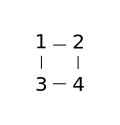
\includegraphics[width=0.32\textwidth]{example_1_res}
        }%
        \subfigure[Matrix with 4 cells]{%
          \label{fig:example_2_matrix}
          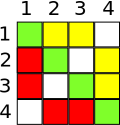
\includegraphics[width=0.32\textwidth]{example_2_matrix}
        }%
        \subfigure[DAG with 4 cells]{%
          \label{fig:example_3_dag}
          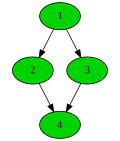
\includegraphics[width=0.32\textwidth]{example_3_dag}
        }%
    \end{center}
    \caption{The red elements determine the dependencies in the DAG.}
    \label{fig:exemple_3_dag}
\end{figure}

So, the parallelism in ILU can be represent under a task form.
%
Each task represents the factorization of one row... which is quite small.
%
In fact, most of task scheduler will take longer to schedule the task than the task takes to factorize a row.



Incomplete factorization and associated triangular solve of a sparse matrix is a problem that is well representative of the difficulty that one can encounter with fine-grain parallelization.
%
The fine grain description of these algorithms is natural, but in practice, a straightforward task based parallelization using TBB or
OpenMP does not deliver good speed-ups because of the very low computational cost of a task.
%
It's called granularity problem.
%
To solve this problem, tasks must become bigger, we need to factorize several rows in one task.
%
But it is not simple to choice which rows could be factorized together without impacting result or parallelism.
%
A generic method has been developed during my thesis and will be explain later in this document.
